
\documentclass[tikz, border=1mm]{standalone}

\usepackage{amsmath}

\usetikzlibrary{calc,angles,quotes,intersections,shapes.geometric}

\usepackage{tkz-euclide}

\begin{document}
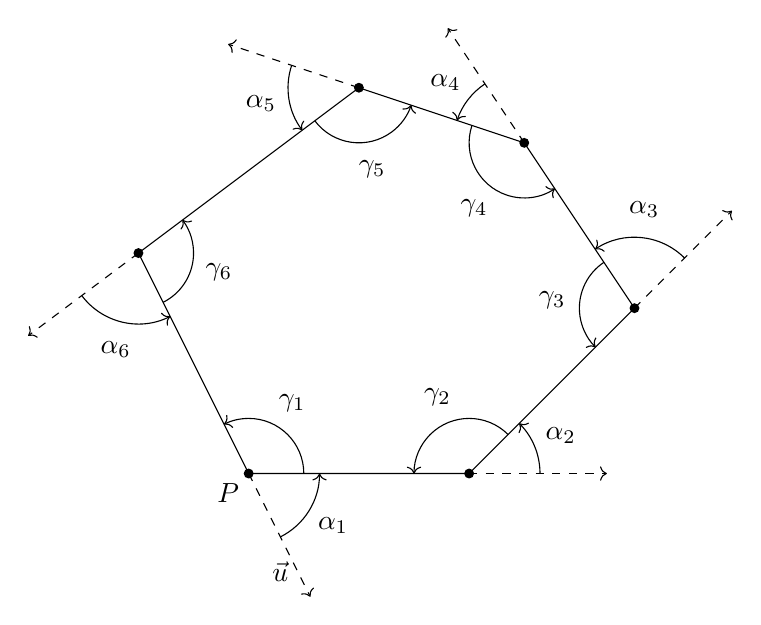
\begin{tikzpicture}[scale=0.7]

	% ---- parameters

	\def\arrowlength{2.5}
	\def\arrowratio{0.6}

	% ---- coordinates

	\coordinate (P1) at (0,0);
	\coordinate (P2) at (4,0);
	\coordinate (P3) at (7,3);
	\coordinate (P4) at (5,6);
	\coordinate (P5) at (2,7);
	\coordinate (P6) at (-2,4);

	% ---- vectors

	\coordinate (v1) at ($ (P1) - (P6) $);
	\coordinate (v2) at ($ (P2) - (P1) $);
	\coordinate (v3) at ($ (P3) - (P2) $);
	\coordinate (v4) at ($ (P4) - (P3) $);
	\coordinate (v5) at ($ (P5) - (P4) $);
	\coordinate (v6) at ($ (P6) - (P5) $);

	% -- unit vectors

	\coordinate (u1) at ($ (0,0)!1cm!(v1) $);
	\coordinate (u2) at ($ (0,0)!1cm!(v2) $);
	\coordinate (u3) at ($ (0,0)!1cm!(v3) $);
	\coordinate (u4) at ($ (0,0)!1cm!(v4) $);
	\coordinate (u5) at ($ (0,0)!1cm!(v5) $);
	\coordinate (u6) at ($ (0,0)!1cm!(v6) $);

	% ---- arrows tips

	% -- fixed length

	\coordinate (A1) at ($ (P1) + \arrowlength*(u1) $);
	\coordinate (A2) at ($ (P2) + \arrowlength*(u2) $);
	\coordinate (A3) at ($ (P3) + \arrowlength*(u3) $);
	\coordinate (A4) at ($ (P4) + \arrowlength*(u4) $);
	\coordinate (A5) at ($ (P5) + \arrowlength*(u5) $);
	\coordinate (A6) at ($ (P6) + \arrowlength*(u6) $);

	% -- proportional length

% 	\coordinate (A1) at ($ (P1) + \arrowratio*(v1) $);
% 	\coordinate (A2) at ($ (P2) + \arrowratio*(v2) $);
% 	\coordinate (A3) at ($ (P3) + \arrowratio*(v3) $);
% 	\coordinate (A4) at ($ (P4) + \arrowratio*(v4) $);
% 	\coordinate (A5) at ($ (P5) + \arrowratio*(v5) $);
% 	\coordinate (A6) at ($ (P6) + \arrowratio*(v6) $);

	% ---- polygon

	\draw (P1) \foreach \i in {2,...,6} { -- (P\i) } -- cycle;

	% ---- arrows

	\draw[dashed, ->] (P1) -- (A1);
	\draw[dashed, ->] (P2) -- (A2);
	\draw[dashed, ->] (P3) -- (A3);
	\draw[dashed, ->] (P4) -- (A4);
	\draw[dashed, ->] (P5) -- (A5);
	\draw[dashed, ->] (P6) -- (A6);

	% ---- thick vertices

	\foreach \i in {1,...,6} { \fill (P\i) circle (0.9mm); }

	% ---- vertices labels

	\node[below left] at (P1) {$P$};

% 	\node[above right] at (P1) {$P_1$};
% 	\node[right] at (P2) {$P_2$};
% 	\node[below] at (P3) {$P_3$};
% 	\node[below] at (P4) {$P_4$};
% 	\node[left] at (P5) {$P_5$};
% 	\node[above left] at (P6) {$P_6$};

	% ---- vectors labels

	\node[left] at ($(P1)!0.8!(A1)$) {$\vec{u}$};

	% ---- angles labels

	\pic[draw, ->, "$\alpha_1$", angle radius=0.9cm, angle eccentricity=1.4]
	{angle = A1--P1--P2};

	\pic[draw, ->, "$\alpha_2$", angle radius=0.9cm, angle eccentricity=1.4]
	{angle = A2--P2--P3};

	\pic[draw, ->, "$\alpha_3$", angle radius=0.9cm, angle eccentricity=1.4]
	{angle = A3--P3--P4};

	\pic[draw, ->, "$\alpha_4$", angle radius=0.9cm, angle eccentricity=1.4]
	{angle = A4--P4--P5};

	\pic[draw, ->, "$\alpha_5$", angle radius=0.9cm, angle eccentricity=1.4]
	{angle = A5--P5--P6};

	\pic[draw, ->, "$\alpha_6$", angle radius=0.9cm, angle eccentricity=1.4]
	{angle = A6--P6--P1};

	\pic[draw, ->, "$\gamma_1$", angle radius=0.7cm, angle eccentricity=1.5]
	{angle = P2--P1--P6};

	\pic[draw, ->, "$\gamma_2$", angle radius=0.7cm, angle eccentricity=1.5]
	{angle = P3--P2--P1};

	\pic[draw, ->, "$\gamma_3$", angle radius=0.7cm, angle eccentricity=1.5]
	{angle = P4--P3--P2};

	\pic[draw, ->, "$\gamma_4$", angle radius=0.7cm, angle eccentricity=1.5]
	{angle = P5--P4--P3};

	\pic[draw, ->, "$\gamma_5$", angle radius=0.7cm, angle eccentricity=1.5]
	{angle = P6--P5--P4};

	\pic[draw, ->, "$\gamma_6$", angle radius=0.7cm, angle eccentricity=1.5]
	{angle = P1--P6--P5};

\end{tikzpicture}
\end{document}
